\newpage
\section{Projektowanie}
\label{sec:projektowanie}

\subsection{Użyte narzędzia i technologie}

W projekcie zastosowane zostały następujące narzędzia i technologie, które wspierają zarówno rozwój aplikacji, jak i zapewniają jej odpowiednią jakość oraz funkcjonalność:

\begin{itemize}
  \item \textbf{Język programowania C++}: Został wybrany ze względu na wysoką wydajność oraz wsparcie dla programowania obiektowego, co umożliwia elegancką implementację algorytmu sortowania przez scalanie oraz operacji na tablicach. C++ jest także powszechnie stosowany w projektach wymagających optymalizacji pamięci i szybkości działania.
  \item \textbf{Google Test}: Framework do testowania jednostkowego, który pozwala na automatyczne sprawdzanie poprawności algorytmu w różnych scenariuszach. Google Test ułatwia również integrację z systemem Continuous Integration (CI), dzięki czemu testy są uruchamiane automatycznie na każdym etapie rozwoju projektu.
  \item \textbf{CMake}: Używany do konfigurowania procesu budowy projektu. CMake generuje odpowiednie pliki dla różnych systemów operacyjnych i kompilatorów, co zapewnia elastyczność przy kompilacji na różnych platformach (Windows, Linux).
  \item \textbf{Ninja}: Lekki system budowania, który jest wykorzystywany razem z CMake do zapewnienia szybciej działających kompilacji. Ninja jest wybierany, ponieważ jest mniej zasobożerny niż tradycyjne systemy budowania.
  \item \textbf{Doxygen}: Narzędzie służące do generowania dokumentacji z komentarzy \\ w kodzie. Doxygen automatycznie tworzy dokumentację w formacie HTML, która jest następnie udostępniana na stronie projektu. Użycie Doxygen pozwala na przejrzystość kodu oraz ułatwia zrozumienie jego działania.
  \item \textbf{GitHub Actions}: Platforma CI/CD umożliwiająca automatyczne uruchamianie testów, generowanie dokumentacji oraz wdrażanie aplikacji na repozytorium GitHub. GitHub Actions jest wykorzystywany do uruchamiania testów jednostkowych, weryfikacji konwencji commitów, generowania dokumentacji oraz publikacji wersji na GitHub Pages.
\end{itemize}

\subsection{Szczegółowe ustawienia kompilatora}

Projekt jest konfigurowany przy użyciu systemu budowania CMake, który generuje odpowiednie pliki konfiguracyjne w zależności od wybranego środowiska. Poniżej przedstawiono szczegóły ustawień kompilatora:

\begin{itemize}
  \item \textbf{Kompilacja dla systemu Linux}: Projekt jest kompilowany za pomocą kompilatora \texttt{g++} (GCC) dostępnego na systemach Linux. Ustawienia CMake są zoptymalizowane pod kątem kompilatora GCC, zapewniając optymalną wydajność podczas kompilacji.
  \item \textbf{Kompilacja dla systemu Windows}: Na systemie Windows projekt jest kompilowany przy użyciu \texttt{MINGW-w64}, który pozwala na kompilację kodu C++ w środowisku zgodnym z GNU (GCC) w systemie Windows. Kompilator ten jest wykorzystywany w połączeniu z MSYS2.
  \item \textbf{Ustawienia CMake}: W projekcie zastosowano plik \texttt{CMakeLists.txt}, który definiuje, jakie biblioteki oraz pliki źródłowe są wykorzystywane w projekcie. Plik konfiguracyjny ustawia również wymagania dotyczące systemu budowania oraz ścieżki do zależności.
  \item \textbf{System Ninja}: W połączeniu z CMake, projekt wykorzystuje system budowania \texttt{Ninja}, który jest lekki i szybki. Dzięki temu proces kompilacji jest szybszy w porównaniu do tradycyjnych systemów, takich jak \texttt{Make}.
\end{itemize}

\subsection{Struktura kodu i diagram klas}

Aby ułatwić zrozumienie struktury aplikacji, na listingu \OznaczZdjecie{uml} przedstawiono diagram klas oraz opis poszczególnych komponentów aplikacji.

\begin{figure}[!htb]
  \begin{center}
    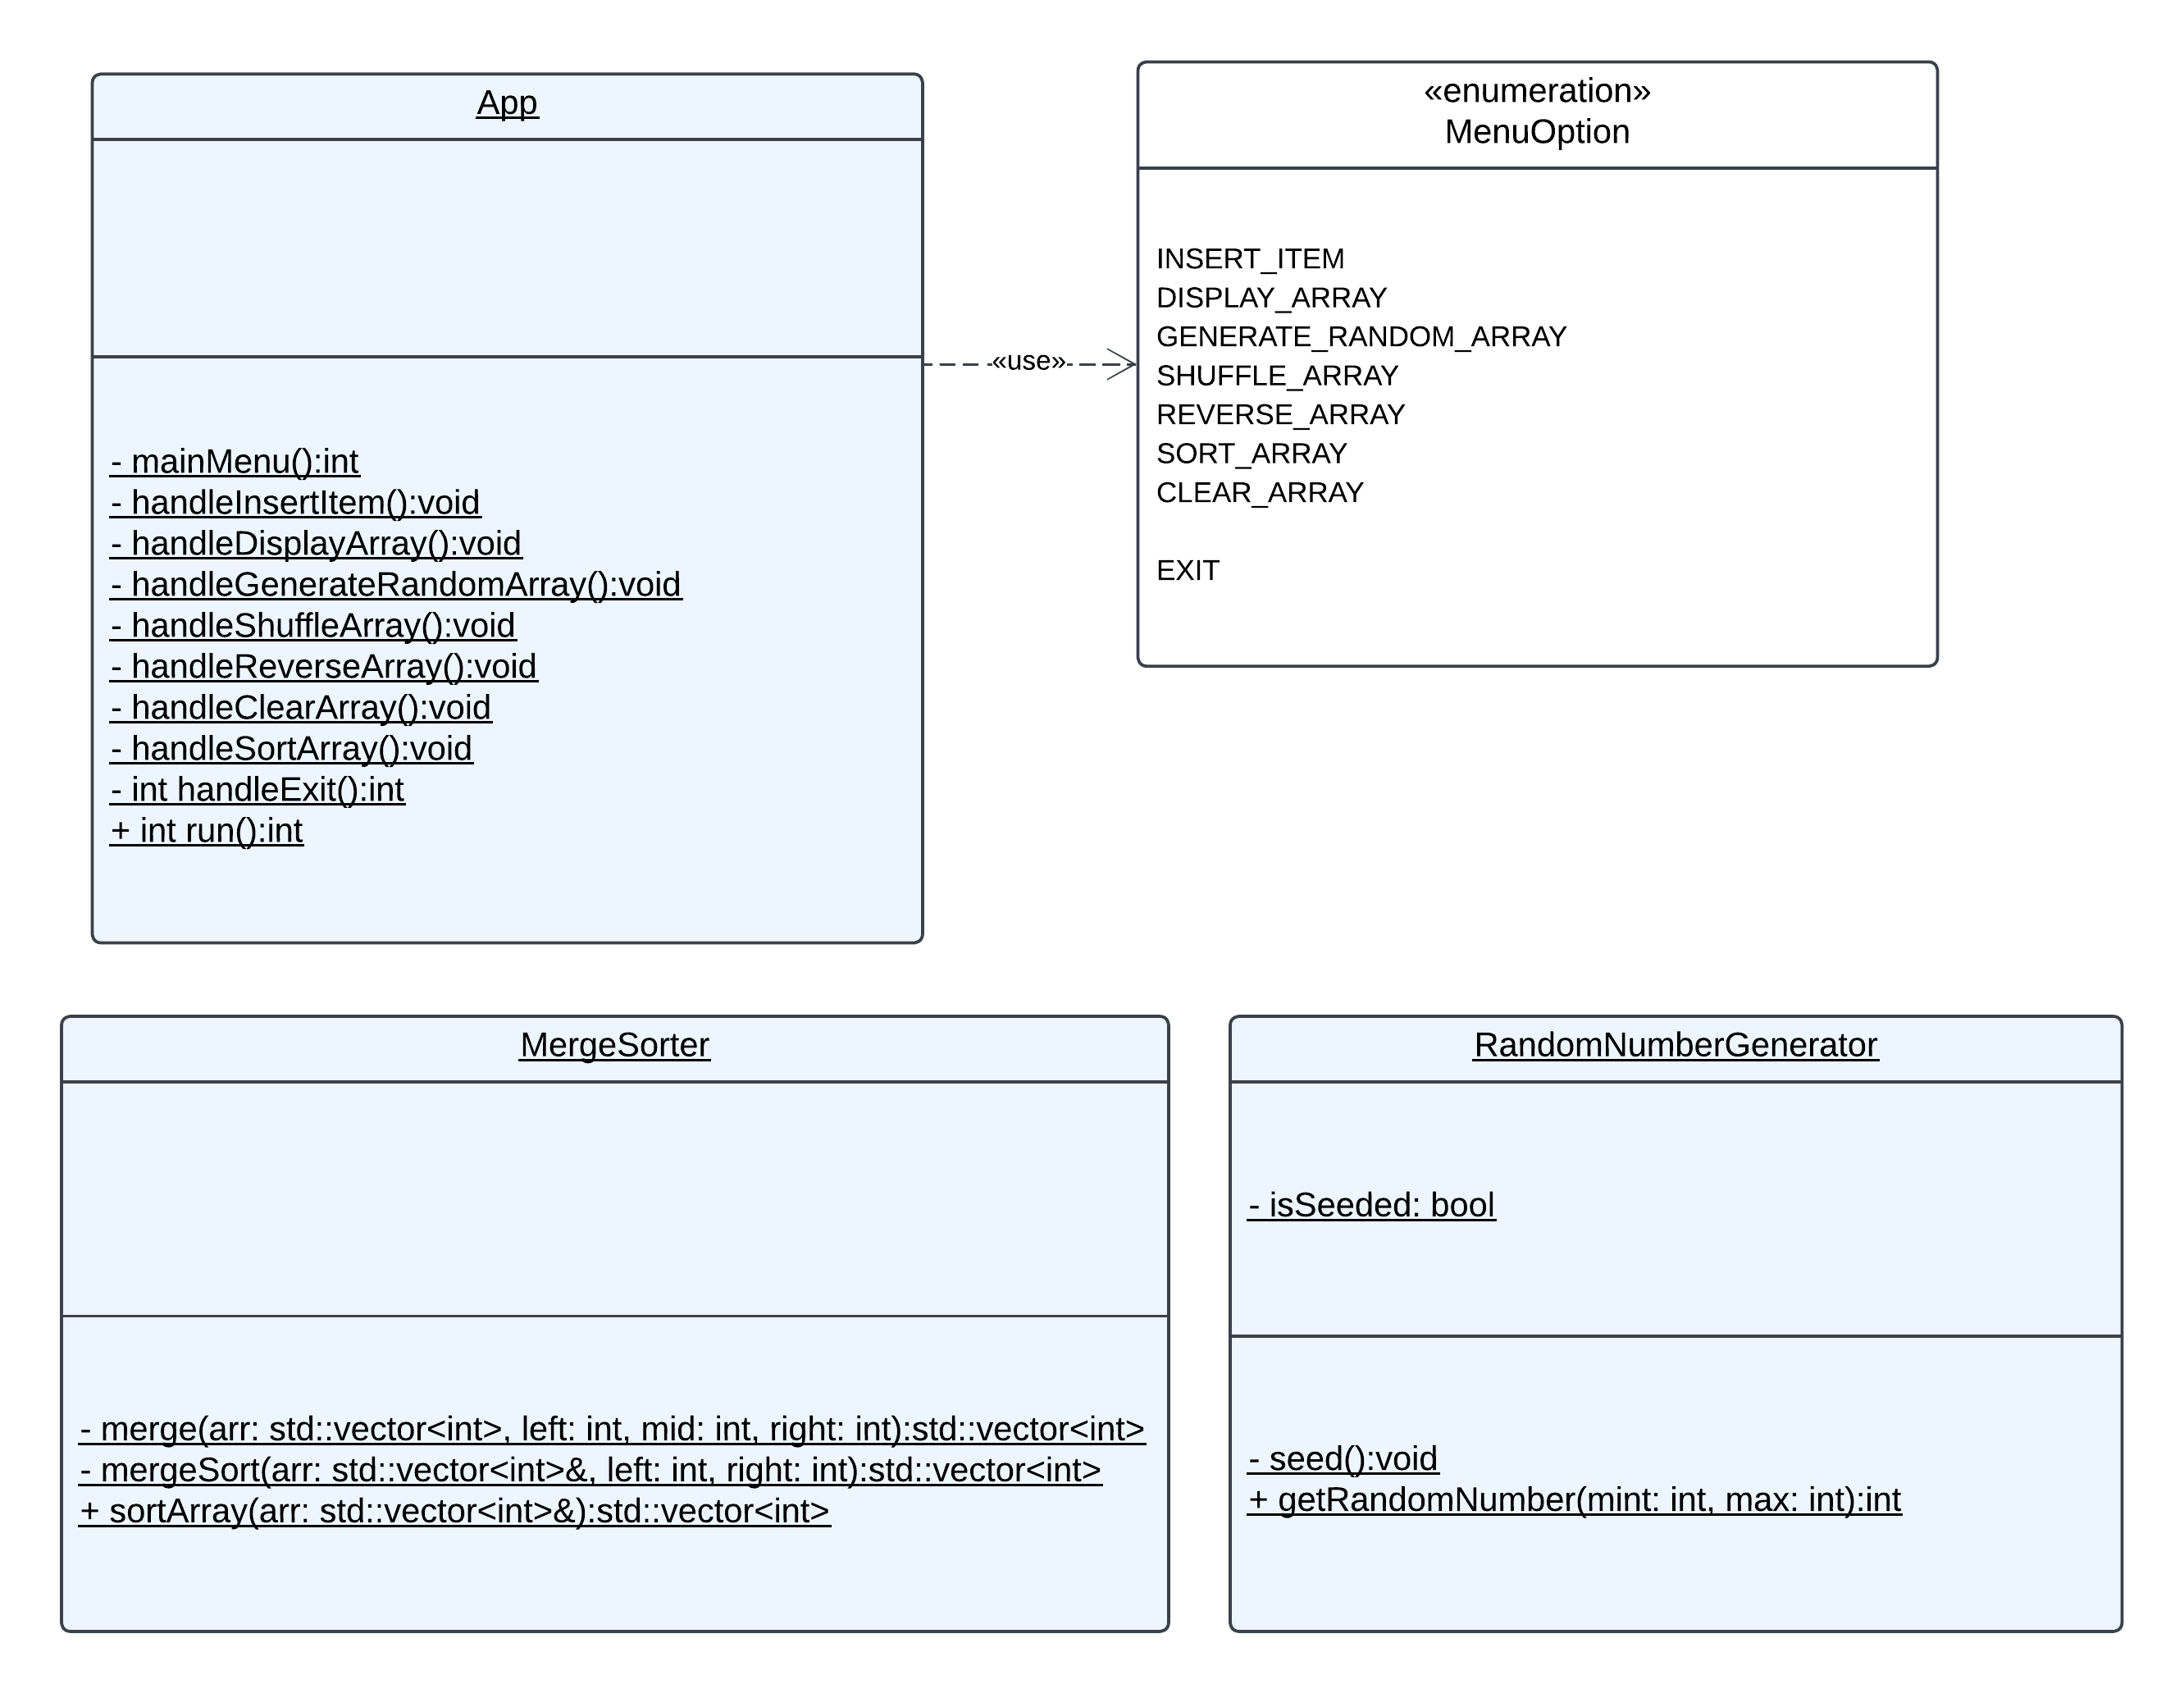
\includegraphics[width=\textwidth]{rys/uml.png}
    \caption{Diagram klas aplikacji MergeSort}
    \label{rys:uml}
  \end{center}
\end{figure}

\textbf{Opis diagramu klas:}

\begin{itemize}
  \item \textbf{App}: Główna klasa aplikacji odpowiedzialna za interakcję z użytkownikiem. Umożliwia wybór różnych operacji na tablicach, takich jak dodawanie, usuwanie, tasowanie i sortowanie.
  \item \textbf{MergeSorter}: Klasa implementująca algorytm sortowania przez scalanie. Zawiera metody odpowiedzialne za dzielenie tablicy, sortowanie oraz scalanie wyników.
  \item \textbf{ArrayUtils}: Biblioteka zawierająca pomocnicze funkcje do manipulacji tablicami, takie jak tasowanie (algorytm Fishera-Yatesa), odwracanie kolejności czy wyświetlanie zawartości tablicy.
  \item \textbf{RandomNumberGenerator}: Klasa generująca losowe liczby całkowite \\ w określonym zakresie. Jest wykorzystywana do generowania danych testowych oraz do inicjalizowania tablic w różnych scenariuszach.
\end{itemize}

\subsection{Schemat działania algorytmu}

Algorytm Merge Sort działa na zasadzie podziału i scalania, co jest kluczowe do zrozumienia jego działania.
Na rysunku \OznaczZdjecie{merge_sort_algorithm} przedstawiono schemat działania algorytmu.

\begin{figure}[!htb]
  \begin{center}
    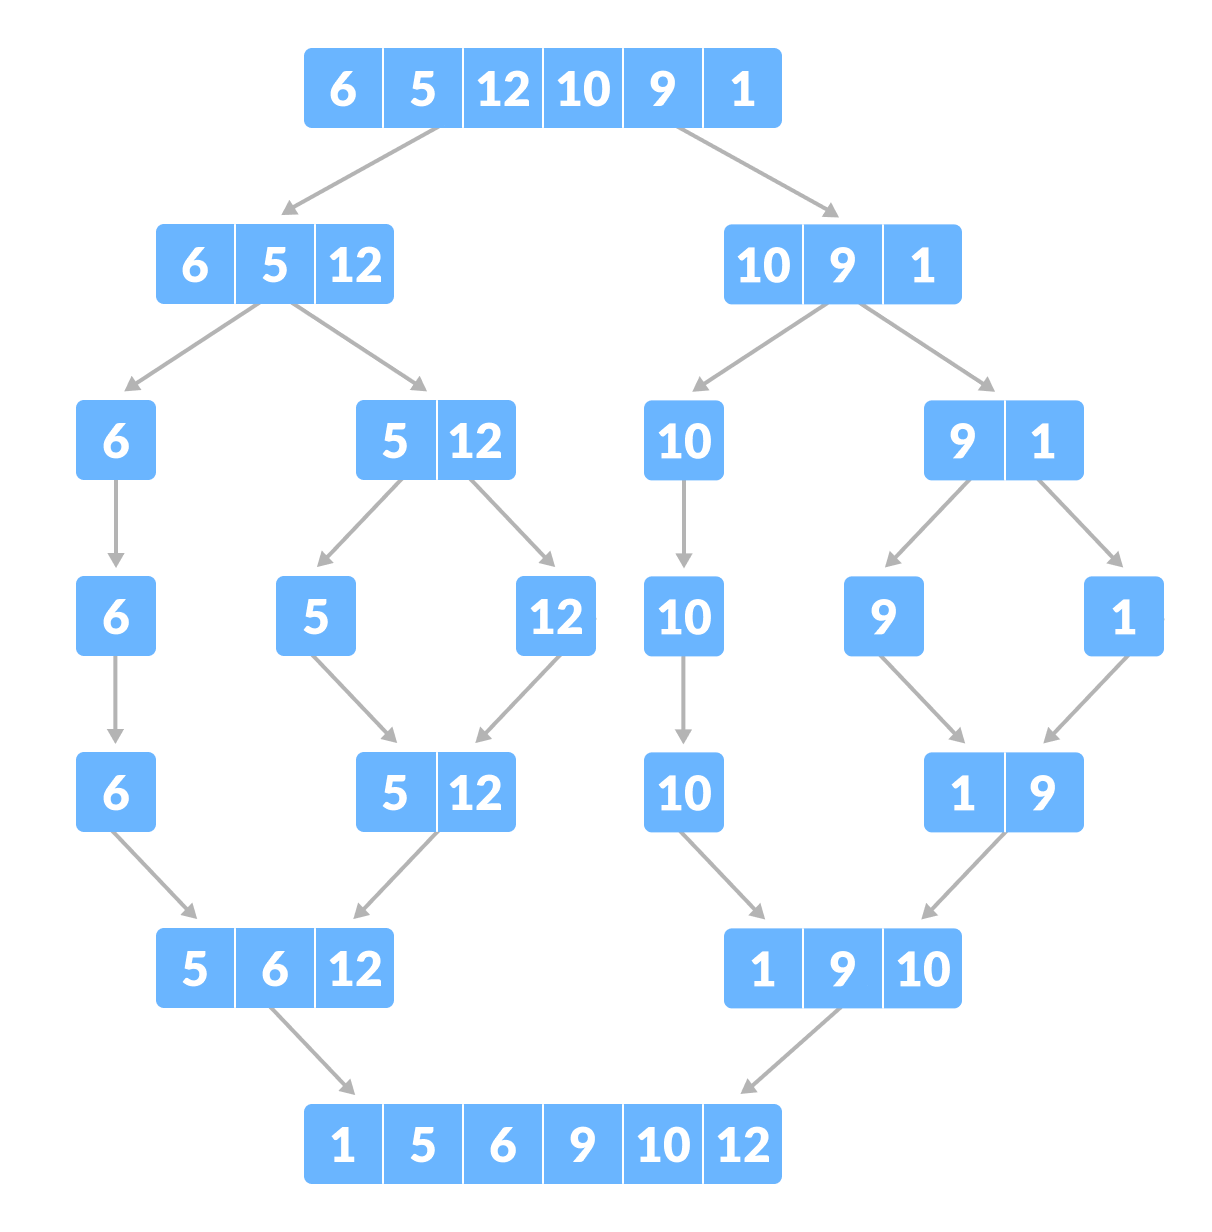
\includegraphics[width=\textwidth]{rys/merge_sort_example.png}
    \caption{Schemat działania algorytmu Merge Sort \protect\footnotemark}
    \label{rys:merge_sort_algorithm}
  \end{center}
\end{figure}

\footnotetext{Źródło: \url{https://www.programiz.com/dsa/merge-sort}}

\textbf{Opis schematu algorytmu:}

\begin{enumerate}
  \item Początkowo tablica jest dzielona na dwie części, aż do uzyskania pojedynczych elementów.
  \item Następnie elementy są scalane w sposób uporządkowany. Scalenie polega na porównaniu pierwszego elementu z obu tablic i wstawieniu mniejszego z nich do nowej tablicy.
  \item Proces ten jest powtarzany, aż wszystkie elementy zostaną scalone w jednej, uporządkowanej tablicy.
\end{enumerate}

\subsection{Zarządzanie wersjami i użycie GIT}

Do zarządzania wersjami kodu wykorzystano system kontroli wersji Git. Projekt jest hostowany na platformie GitHub, gdzie korzysta się z następujących funkcji:

\begin{itemize}
  \item \textbf{Branching}: Rozwój projektu odbywa się na osobnych gałęziach, co pozwala na wprowadzenie nowych funkcji lub poprawek bez wpływu na główną wersję projektu (gałąź \texttt{main}).
  \item \textbf{Pull Requests}: Zmiany wprowadzane na gałęziach są łączone z główną gałęzią poprzez pull requesty, co umożliwia przeglądanie kodu oraz automatyczne uruchamianie testów przed połączeniem zmian.
  \item \textbf{Commit Hooks}: Zastosowanie \texttt{Git Hooks} umożliwia automatyczne uruchamianie testów jednostkowych przed każdą zmianą w repozytorium, co zapewnia, że tylko poprawny kod zostanie zaakceptowany.
  \item \textbf{GitHub Actions}: Zautomatyzowane procesy CI/CD pozwalają na uruchamianie testów, generowanie dokumentacji oraz publikację wyników na GitHub Pages.
\end{itemize}

\subsection{Testy jednostkowe}

Testy jednostkowe są kluczowym elementem procesu weryfikacji poprawności działania algorytmu Merge Sort. Celem testów jest zapewnienie, że implementacja algorytmu działa zgodnie z oczekiwaniami w różnych scenariuszach, a także wykrywanie potencjalnych błędów w kodzie. W projekcie zastosowano framework \texttt{Google Test}, który pozwala na pisanie i uruchamianie testów w sposób automatyczny. Poniżej przedstawiono szczegóły dotyczące testów jednostkowych.

\subsubsection{Przykłady testów jednostkowych}

Testy jednostkowe w projekcie obejmują szeroki zakres przypadków testowych, mających na celu sprawdzenie poprawności algorytmu Merge Sort w różnych warunkach. Poniżej przedstawiono kilka przykładów testów:

\begin{itemize}
  \item \textbf{Testowanie tablicy już posortowanej}: Sprawdzany jest przypadek, gdy algorytm otrzymuje już posortowaną tablicę. Oczekiwany wynik to ta sama tablica, ponieważ algorytm nie powinien wprowadzać żadnych zmian w takim przypadku.
  \item \textbf{Testowanie tablicy w odwrotnej kolejności}: Testuje się przypadek, gdy tablica jest posortowana w odwrotnej kolejności. Merge Sort powinien prawidłowo posortować tę tablicę w porządku rosnącym.
  \item \textbf{Testowanie tablicy z duplikatami}: Sprawdzany jest przypadek, w którym tablica zawiera elementy powtarzające się. Algorytm powinien poprawnie poradzić sobie z duplikatami, zachowując ich obecność w posortowanej tablicy.
  \item \textbf{Testowanie tablicy z liczbami ujemnymi}: Algorytm jest testowany \\ w sytuacji, gdy tablica zawiera liczby ujemne. Oczekiwany wynik to posortowanie tych liczb w porządku rosnącym.
  \item \textbf{Testowanie dużych tablic}: Sprawdzany jest przypadek, gdy tablica zawiera dużą liczbę elementów (np. 1000 lub więcej). Algorytm powinien działać wydajnie, bez przekroczenia limitów czasowych i pamięciowych.
\end{itemize}

\newpage

\subsubsection{Struktura testów jednostkowych}

Wszystkie testy jednostkowe zostały zorganizowane w oddzielnym pliku \texttt{merge\_sorter\_test.cpp}. Każdy test sprawdza określoną funkcjonalność algorytmu, a wyniki testów są raportowane za pomocą frameworka \texttt{Google Test}, który automatycznie generuje raporty o wynikach każdego z testów.

Przykład testu jednostkowego w projekcie:

\lstinputlisting[caption=Przykład testu jednostkowego, label={lst:example_test}, language=C++]{kod/example_test.cpp}

W przykładzie pokazanym na listingu \OznaczKod{example_test} testowana jest tablica, która już jest posortowana. Algorytm Merge Sort powinien zwrócić tę samą tablicę. Funkcja \texttt{EXPECT\_EQ} sprawdza, czy wynik sortowania jest zgodny z oczekiwanym.

\subsubsection{Integracja testów z systemem CI/CD}

Testy jednostkowe są integralną częścią procesu Continuous Integration (CI), co oznacza, że są one automatycznie uruchamiane za każdym razem, gdy kod jest zmieniany i wysyłany do repozytorium. Dzięki integracji z \texttt{GitHub Actions}, każda zmiana w kodzie uruchamia zestaw testów jednostkowych, weryfikując poprawność nowego kodu przed jego połączeniem z główną gałęzią projektu.

\begin{itemize}
  \item \textbf{Automatyczne uruchamianie testów}: Testy są uruchamiane automatycznie na każdej gałęzi projektu, a wyniki są raportowane na platformie GitHub. Dzięki temu deweloperzy mogą natychmiast zobaczyć, czy ich zmiany wprowadzają jakiekolwiek błędy.

        \begin{figure}[!htb]
          \begin{center}
            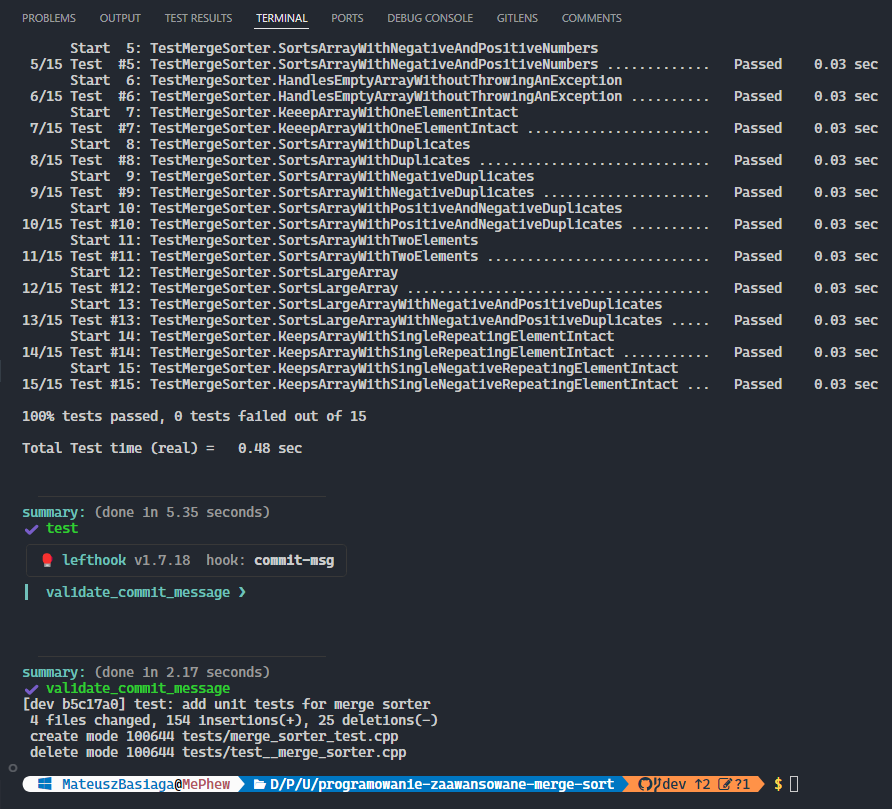
\includegraphics[width=\textwidth]{rys/tests_pre_commit.png}
            \caption{Przykładowy przebieg testów po wykonaniu commita}
            \label{rys:tests_pre_commit}
          \end{center}
        \end{figure}

        Na rysuku \OznaczZdjecie{tests_pre_commit} pokazano przebieg testów uruchomiony automatycznie po wykonaniu commita.
        Aby commmit został wykonany wynik testów musi być pozytywny.

  \item \textbf{Przegląd wyników testów}: Każdy commit generuje raport o wynikach testów, który jest dostępny na stronie z historią commitów. Umożliwia to szybkie wykrycie błędów w kodzie oraz ich naprawienie.
  \item \textbf{Zabezpieczenie przed błędami}: Każda próba połączenia kodu z gałęzią \texttt{main} wymaga, aby testy jednostkowe zakończyły się sukcesem. Dzięki temu, kod w głównej gałęzi projektu zawsze jest sprawdzony i działa zgodnie z oczekiwaniami.
\end{itemize}
